\documentclass{jarticle}
% \usepackage{flushend}  % 最終ページの2カラムの左右の高さを揃える
\usepackage[dvipdfmx]{graphicx}
\usepackage{subcaption}
\captionsetup[figure]{justification=centering}
\captionsetup[table]{justification=centering}
\usepackage[ipa]{pxchfon}
\usepackage{otf}
\renewcommand{\figurename}{図~}
\renewcommand{\tablename}{表~}
\newcommand{\figref}[1]{\figurename\ref{#1}}
\newcommand{\tabref}[1]{\tablename\ref{#1}}
\usepackage{robomech}
% \usepackage[dvipdfmx,setpagesize=false]{hyperref}



\begin{document}
\makeatletter
\title{視覚と行動のend-to-end学習により\\経路追従行動をオンラインで模倣する手法の提案}
{― データセット収集密度の動的調整による学習の効率化 ―}
{A proposal for an online imitation method of
path-tracking\\ behavior by end-to-end learning of vision and action}
{- Efficiency improvement of learning by dynamic adjustment of dataset collection density -}

\author{
\begin{tabular}{c}
 \hspace*{0.3zw}○学\hspace{1zw}今井悠月 (千葉工大)\hspace{2zw}正\hspace{1zw}上田隆一 (千葉工大)\hspace{2zw}正\hspace{1zw}林原靖男(千葉工大)\\
 \end{tabular}
 \vspace{1zh} \\
 \begin{tabular}{l}
 {\hspace*{4zw}\small Yuzuki IMAI, Chiba Institute of Technology, s20c1015as@s.chibakoudai.jp}\\
 {\hspace*{4zw}\small Ryuichi UEDA, Chiba Institute of Technology}\\
 {\hspace*{4zw}\small Yasuo HAYASHIBARA, Chiba Institute of Technology}\\
\end{tabular}
}
\makeatother

\abstract{ \small 
Our objective is to diversify the navigation methods in autonomous mobile robots. To achieve this, we have proposed a method that uses end-to-end learning of images and angular velocity to follow a path. This method involves collecting a dataset while the robot is in operation and using it for learning. However, the translational speed has not been discussed so far, and there is a possibility that data has been over-collected in some parts of the route. As a result, some data may not be learned, leading to a potential failure in path-following. Therefore, this paper first elucidates whether the cause of path-following failure is due to an imbalance in the dataset. Subsequently, we propose a method to adjust the data collection density by varying the translational speed of the robot, and we verify its effectiveness through experiments using a simulator.
}

\date{} % 日付を出力しない
\keywords{Navigation,  Autonomous mobile robot,  End-to-end learning,  Dataset}

\maketitle
\thispagestyle{empty}
\pagestyle{empty}

\small
\section{緒言}
本研究グループは,移動ロボットにおけるナビゲーション手段の複数化を目標としている.その目標を達成するため,
従来からカメラ画像とロボットの角速度を end-to-end 学習することで,経路追従する手法を提案し,その有効性を
検証してきた\cite{okada}\cite{okada2}\cite{kiyooka}.
本手法は,複数のセンサと地図を入力として生成した行動を,画像を入力とする行動に模倣する.これによりロボット
は,複数のセンサと地図を使用した時と同じ行動を,画像のみで行えるようになる.よって,地図に基づく経路追従と
画像に基づく経路追従の 2 つのナビゲーション手段を獲得できる.これらを状況に応じて高い信頼性が見込まれる方
を選択することで,経路追従を継続できる可能性が高まる.\\
\hspace*{1zw}本研究と同様に,カメラ画像を入力として,end-to-end 学習により経路追従する手法は,いくつか
提案されている.
例えば,Muller らは,人のコントローラ操作と画像を end-to-end 学習することで,オフロード環境で障害物を
回避して走行できることを確認した\cite{off_load}.また,Moridian らは,人のコントローラ操作と画像,測域
センサのデータを end-to-end 学習することで,一定の経路を走行できることを確認した\cite{Moridian}.
さらに,Bojarski らは,画像と人が操作したステアリングの角度を end-to-end 学習することで,自動運転する
手法を提案した\cite{Bojarski}.
これらの手法はすべて人の操作を教師データとしているのに対し,本手法はルールベースの制御器の出力である
角速度を教師データとしている.そのため,データセットの収集に人の操作が不要である.
それに加えて,ロボットが目標経路に復帰する行動を収集できるため,経路追従の継続に有効であることが確認
されている\cite{imai}.\\
\hspace*{1zw}ここで,本手法はロボットを走行させながらデータセットを収集し,それを用いて学習するが,
ロボットの並進速度に関してはこれまで議論されていない.
従来は,常に一定の速度(0.2 m/s)でロボットを走行させていたが,経路の一部で必要以上にデータを収集している
おそれがある.
収集したデータセットの順序は,各ステップ(0.2 s 程度)ごとに無作為に並び替えられ,その中の一部を学習に
用いるため,割合の多いデータは多く学習され,割合の少ないデータはあまり学習されていない可能性がある.
経路の一部でも学習が不足すると,ロボットは経路追従できないため,データの収集密度を改善し,
学習に用いられるデータの偏りを少なくすることが望まれる.\\
\hspace*{1zw}これを踏まえ,本稿では,まず従来手法における経路追従失敗の一例を取り上げ,
その要因がデータセットの不均衡によるものであるかを明らかにする.
そのうえで,ロボットの並進速度を教師データの値に応じて可変にすることで,データセットの
収集密度を調整し,学習を効率化する手法を提案する.
なお,このような学習を効率化する手法は,これまでに本研究グループでもいくつか提案されている.
例えば,藤原らは,オーバーサンプリングによりデータの不均衡を改善する手法を提案した\cite{fuji}.
また,\CID{8705}橋らは,データを事前に収集し,オフラインで学習する手法を提案した\cite{takahashi}.
さらに,今井らは,モデルの評価に基づき訓練を打ち切る手法を提案した\cite{imai2}.
いずれの手法も訓練時間の短縮に成功しているが,本稿における提案手法とはアプローチが異なる.\\
\hspace*{1zw}本稿では,今井らの手法を採用し,シミュレータで実験する.
ロボットの並進速度を可変にする場合と,そうでない場合で結果を比較することにより,
提案手法の有効性を検証する.


\section{end-to-end学習により経路追従行動を模倣する手法}
本研究グループが従来から提案する手法について述べる.本手法は,\figref{fig:1}に示すように,
64×48にリサイズした画像を入力,ロボットの角速度を出力として, end-to-end で学習する.
なお,一定時間(0.2 s 程度)ごとにデータセットを収集しつつ,学習するが,これを 1 ステップとしている.
1 ステップにつき,画像と角速度をペアにしたデータセットの中から 8 個のデータを抽出し,それ用いて学習する.
ただし,過学習を防ぐために,データセットの順序は 1 ステップごとに入れ替わる.
よって,学習に用いられるデータは,毎回で異なる.
ネットワークは \figref{fig:2} に示すように,
左から順に,入力層 1 ,畳み込み層 3 ,全結合層 2 ,出力層 1 の全 7 層で構成される.
また,本手法は,学習時と学習後でシステムが異なる.以下に,それぞれの構成を述べる.


\begin{figure}[h!]
  \centering
   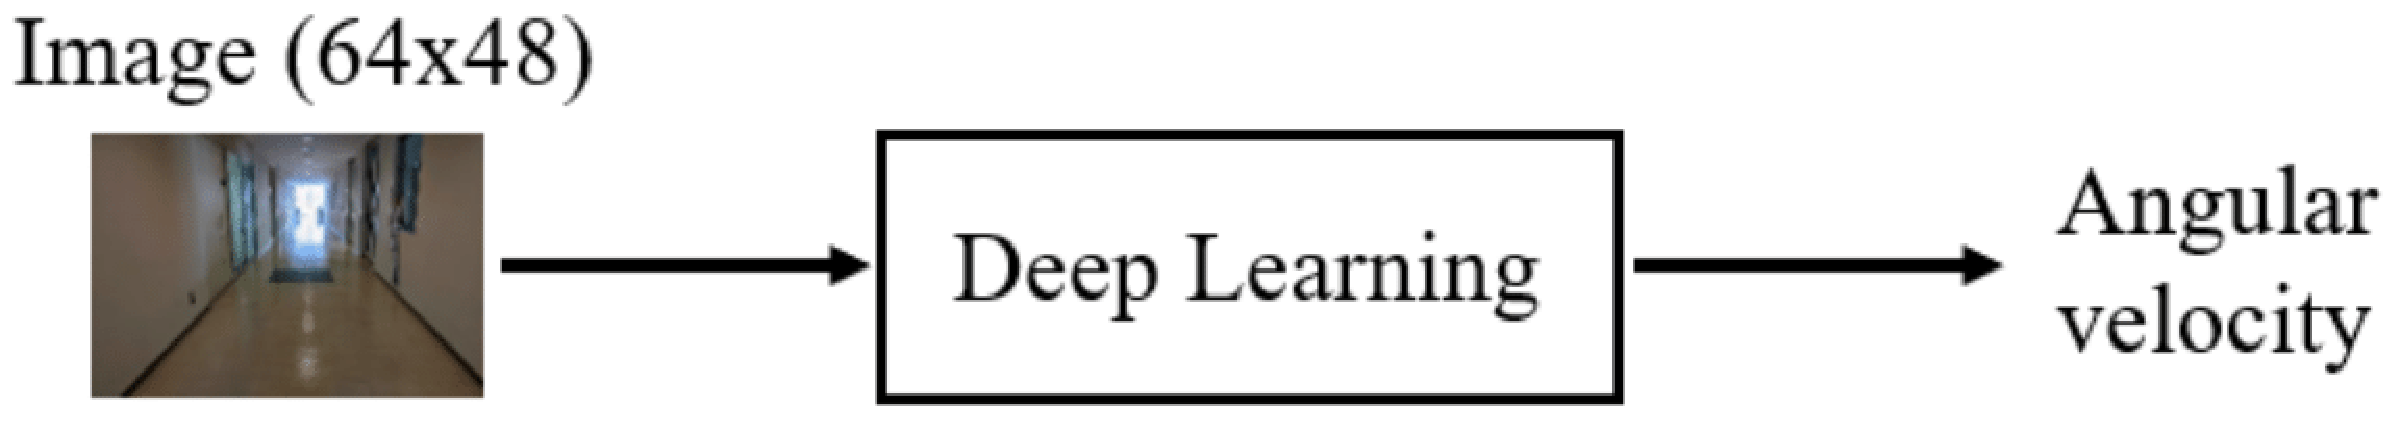
\includegraphics[height=15.5mm]{./pdf/deplearning1.pdf}
   \caption{The end-to-end learning method}
   \label{fig:1}
\end{figure}

\newpage

\begin{figure}[h!]
  \centering
   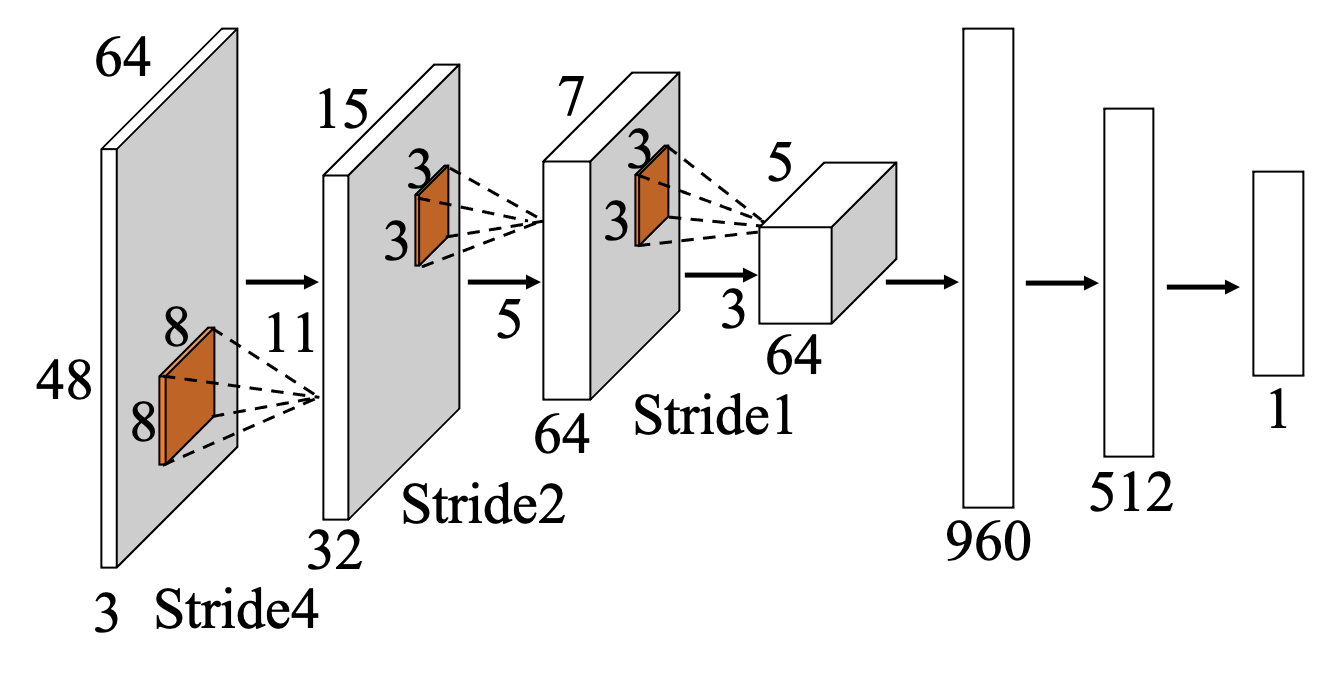
\includegraphics[height=43mm]{pdf/network.pdf}
   \caption{Structure of network}
   \label{fig:2}
\end{figure}


\subsection{地図に基づく経路追従の模倣学習}
地図に基づく経路追従とは,あらかじめ作成した地図と LiDAR,オドメトリなどを用いて,
自己位置推定,経路計画,制御などの複数のタスクを実行し,経路追従する方法である.
ここで,地図に基づく経路追従を模倣学習するシステムを\figref{fig:3}に示す.
学習時には,ルールベースの制御器となる ROS navigation パッケージ\cite{navigation}を用いて,ロボットは
自律移動する.それと同時に,画像と ROS navigation パッケージから出力される
ヨー方向の目標角速度をペアにしたデータセットを収集し,end-to-end で学習する.
ROS navigation パッケージは,並進速度と角速度を出力するが,角速度のみを教師データとし,
並進速度は常に一定(0.2 m/s)とする.
なお,他の研究\cite{Moridian}\cite{Bojarski}に倣い,データセットの収集には 3つのカメラ(左・中央・右)
を用いる.
この時,\tabref{table:1}のように,左右のカメラ画像に対応する目標角速度には,
それぞれ目標経路に戻るようにオフセットを加える.
具体的には,左のカメラには目標角速度に 0.2 rad/s を引いた値を,
右のカメラには目標角速度に 0.2 rad/s を足した値を教師データとする.
これにより,データの量を増やすことや,過学習を防ぐ効果が期待される.
ただし,旋回時(0.1 rad/s 以上)には,中央のカメラのみを使用する.
ロボットのモータを制御するモジュールは,ROS  navigation パッケージから出力される
角速度と,学習器から出力される角速度の 2つで構成されており,この 2つを切り替えることが可能である.
学習器の出力をベースに走行すると,学習ができていない部分でロボットは目標経路から外れることになるため,
目標経路へ復帰する行動をより効率的に収集できる.

\begin{figure}[h!]
  \centering
   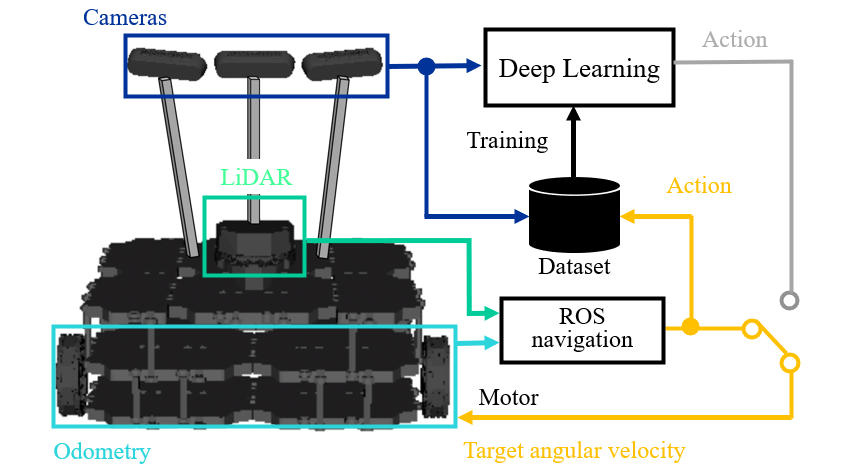
\includegraphics[height=50mm]{./png/learn.png}
   \caption{Method to imitate path-tracking behavior}
   \label{fig:3}
\end{figure}


\begin{table}[h!]
  \centering
  \caption{Yaw angular velocity offset per camera}
  \label{table:1}
    \scalebox{0.90}[0.90]{
    \begin{tabular}{|l||l|}
      \hline
      Cameras & Yaw angular velocity offset (rad/s)\\
      \hline\hline
      Left camera & ROS navigation system output $-$ 0.2\\
      \hline
      Center camera & ROS navigation system output\\
      \hline
      Right camera & ROS navigation system output $+$ 0.2\\
      \hline
    \end{tabular} }
\end{table}

\subsection{訓練済みモデルを用いた視覚に基づく経路追従}
学習が終了したら,訓練済みモデルを用いて,経路追従できるかを確認する.
このときのシステムを\figref{fig:4}に示す.
ここでは,ROS の navigation パッケージからの出力は使用せずにロボットを制御する.
地図に基づく経路追従の模倣学習時と同様に,画像を学習器に入力し,その推定結果をヨー方向の
目標角速度としてロボットを自律移動させる.
ロボットのヨー方向の角速度には学習器の出力を用いるが,並進速度は常に一定 (0.2 m/s) とする.
また,地図に基づく経路追従の模倣学習時には, 3 つのカメラ(左・中央・右)を用いたが,
訓練済みモデルを用いた視覚に基づく経路追従時には, 3 つのカメラのうち,中央のカメラのみを使用する.

\begin{figure}[h!]
  \centering
   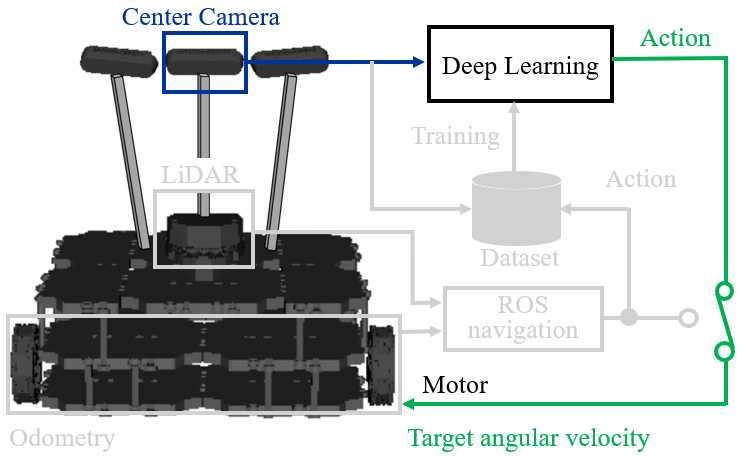
\includegraphics[height=49mm]{./png/afterlearn.png}
   \caption{Vision-based path-tracking using learned model}
   \label{fig:4}
\end{figure}

\section{モデルの評価に基づき訓練を打ち切る手法}
本稿の実験で採用する,今井らが提案した手法について述べる.\figref{fig:5}に本手法のシステムを示す.
2.1節で述べた地図に基づく経路追従の模倣学習手法に,訓練中のモデルを評価し,
望む出力がある程度得られたと判定したら,訓練を終了する仕組みを追加している.
具体的には,ROS navigation パッケージの出力である角速度と,学習器の出力である角速度を比較する.
比較の結果,その差の絶対値が一定値(0.05 rad/s)未満であれば,その地点において望ましい出力が得られている
と判定する.この点を DOL(desired output location)と呼び,判定をステップごとに繰り返す.
データセットを収集しつつ,学習し, DOL の割合が一定値を超えたところで訓練を打ち切る.
これにより,従来は一定のステップ数を用いていた訓練を,訓練の結果に応じて適切なステップ数で打ち切る.
ただし,経路の一部でも DOL が少ないと経路追従できないため,DOL の割合は経路全体に対して
ではなく,経路を分割して算出することが望ましい.今井らは,DOL の算出を各経由点間で行っていたが,
経由点の配置はヒューリスティックに決定されるため,公平な算出方法とはいえない.
DOL の公平な算出方法については今後の課題とし,本稿では議論しないこととする.
以降,本手法を従来手法と呼ぶこととする.

\begin{figure}[h!]
  \centering
   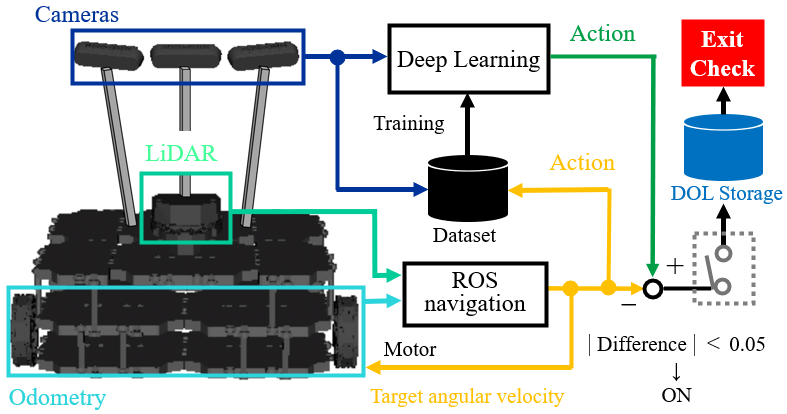
\includegraphics[height=47mm]{./png/moderu.png}
   \caption{Method to terminate training}
   \label{fig:5}
\end{figure}

\newpage

\section{従来手法を用いた経路追従の失敗要因の解析}
従来手法では,すべての経由点間で DOL の割合が 33 %以上 であれば,99%経路追従に成功する
ことが確認されている\cite{imai2}.
ただし,訓練を打ち切る基準を満たしていても経路追従に失敗する例がある.
失敗の要因としては,データセットの不均衡が考えられる.
各経由点間で基準を満たしても,すべての経由点間で基準を満たすまでは学習が継続されるため,
割合の多いデータが多く学習されることで,モデルのパラメータが偏る可能性がある.
そこで,再現実験を行い,それによって得た経路追従失敗の一例から要因を解析する.

\subsection{実験装置}
実験はシミュレータで行う.シミュレータには Gazebo\cite{gazebo},環境には Willow Garage を用いた.
ロボットには TurtleBot3\cite{TurtleBot3}にカメラを 3つ取り付けたモデルを用いた.

\subsection{実験方法}
実験では,はじめに地図に基づく経路追従を模倣学習する.
このとき,ロボットは\figref{fig:6}に示すような緑色の経由点を順次移動するが,
経由点の配置は先行研究と同じである.
ここで,どの地点で得られたデータがどの程度収集されたかを確認するため,
各経由点間に位置情報を加えたデータセットを収集する.
図の赤で示した部分は,先行研究において経路追従に多く失敗した地点であることを意味する.
ただし,ロボットは位置情報は学習せず,従来と同様に画像から角速度のみを予測する.
学習後は,視覚に基づく経路追従で,経路を 1 周できるか確認する.
壁に衝突することなく 1 周できれば経路追従に成功したと判断する.
実験は,経路追従の失敗例を確認するまで行う.
その後,経路追従失敗時のデータを用いて失敗の要因を解析する.

\begin{figure}[h!]
  \centering
   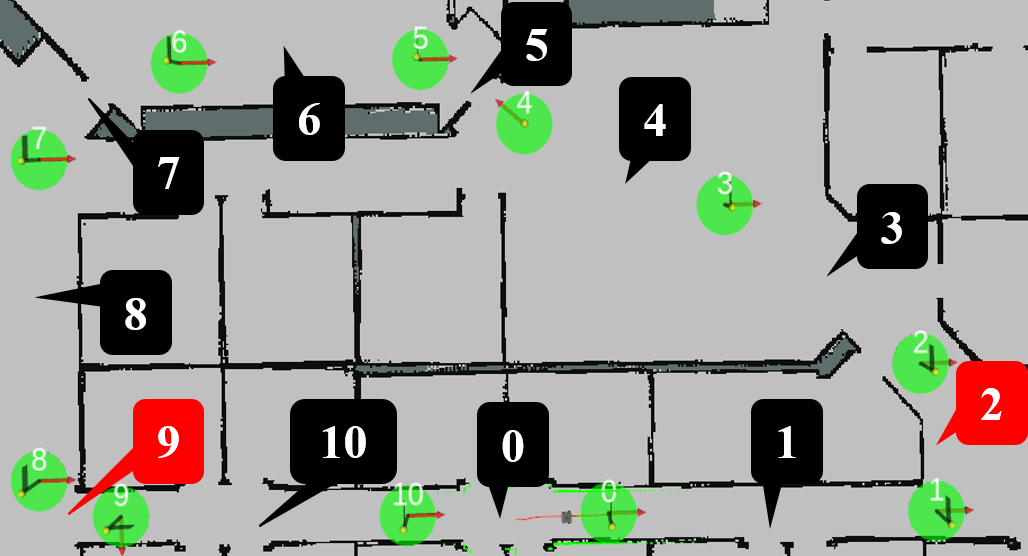
\includegraphics[height=40mm]{./png/location.png}
   \caption{Waypoints used in the experiment}
   \label{fig:6}
\end{figure}

\subsection{実験結果}
経路追従失敗の一例を\figref{fig:7}に示す.ロボットは,左下の曲がり角で壁に衝突した.
この地点は,\figref{fig:6}の 9 番に該当する.ここで,収集したデータセットの割合を\figref{fig:8},
学習に用いられたデータセットの割合を\figref{fig:9}に示す.
\figref{fig:8}より,経路追従に失敗した地点である 9 番のデータセットが他の地点と比べて少ないことがわかる.
また,\figref{fig:9}より,0 番や 1 番など,直線部のデータが多く学習され,9 番のデータセットがあまり学習
されていないことがわかる.
このように,収集したデータセットに偏りがあると,学習されるデータセットも偏る.
これらの結果から,経路追従の失敗要因はデータセットの不均衡によるものであるといえる.

\begin{figure}[h!]
  \centering
   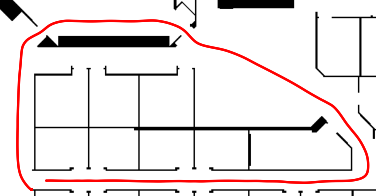
\includegraphics[height=30.3mm]{./png/failed.png}
   \caption{Robot trajectory in the experiment}
   \label{fig:7}
\end{figure}

\newpage

\begin{figure}[h!]
  \centering
   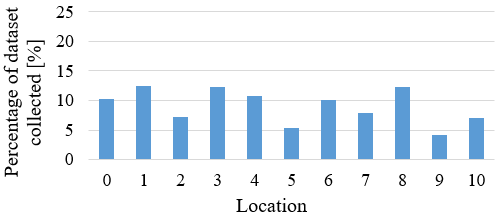
\includegraphics[height=32.8mm]{./png/set2.png}
   \caption{Precentage of dataset collected}
   \label{fig:8}
\end{figure}

\begin{figure}[h!]
  \centering
   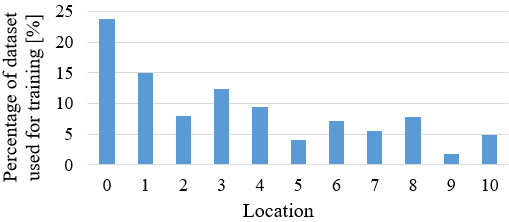
\includegraphics[height=32.8mm]{./png/gaku2.png}
   \caption{Precentage of dataset used for training}
   \label{fig:9}
\end{figure}


\section{提案手法}
4章の結果から,経路追従失敗の要因はデータセットの不均衡によるものであることが確認された.
よって,データセットの収集密度を調整する手法を提案する.
\figref{fig:10}に提案手法を示す.従来手法では,学習時のロボットの並進速度は常に一定(0.2 m/s)
であったが,教師データとなる ROS navigation パッケージの目標角速度の値に応じて
ロボットの並進速度を可変にする仕組みを追加している.具体的には,目標角速度の絶対値が 0.1 rad/s 未満
であれば,ロボットの並進速度を従来の2倍(0.4 m/s)とし,0.1 rad/s 以上であれば,従来と同じ(0.2 m/s)
とする.なお,0.1 rad/s という値は,3つのカメラを用いるしきい値に由来する.
これにより,経路内の直線部などのデータを必要以上に収集することを防ぐ効果が期待される.
また,データセットの不均衡が改善されることで,訓練打ち切りの指標を比較的早い段階で満たすことが
できると考えられる.


\begin{figure}[htbp]
  \begin{minipage}[t]{0.5\linewidth}
    \centering
    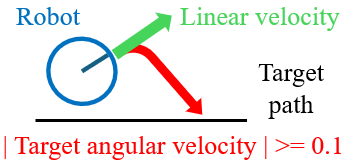
\includegraphics[keepaspectratio, scale=0.33]{./png/a.png}
    \subcaption{Not change linear velocity}
  \end{minipage}
  \begin{minipage}[t]{0.5\linewidth}
    \centering
    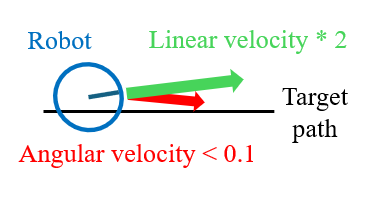
\includegraphics[keepaspectratio, scale=0.33]{./png/b.png}
    \subcaption{Change linear velocity}
  \end{minipage}
  \caption{Proposed method}
  \label{fig:10}
\end{figure}


\section{提案手法を用いた実験}

\subsection{実験装置,実験方法}
提案手法の有効性を検証するため,実験を行う.
実験装置や実験方法は 4章と同様であるが,失敗の有無にかかわらず,100 回実験する.
経路追従の成功率と訓練打ち切りステップ数,データセットの割合から提案手法の有効性を評価する.

\subsection{実験結果}
\subsubsection{経路追従の成功率}
\tabref{table:2}に経路追従の結果を示す.
結果的に,提案手法を用いても,従来手法と経路追従の成功率は変わらなかった.
ちなみに失敗した 1 回は,4.3節の\figref{fig:7}と同じ場所であった.

\newpage

\begin{table}[h!]
  \centering
  \caption{Number of successes in experiments}
  \label{table:2}
    \scalebox{0.90}[0.90] {
    \begin{tabular}{|l||c|}
      \hline
      Experiments & Number of successes \\
      \hline\hline
      Conventional method & 99/100 \\
      \hline
      Proposed method & 99/100\\
      \hline 
    \end{tabular} }
\end{table}

\subsubsection{訓練打ち切りステップ数}
\figref{fig:11}に,訓練打ち切りステップ数の分布を示す.
結果的に,提案手法を用いた方が訓練打ち切りの指標を早くに満たすことができるといえる.
ちなみに,従来手法の平均ステップ数は約 6262ステップ,提案手法の平均ステップ数は
約 4742ステップであり,平均で約 1500ステップ(約5分)の訓練時間を短縮できた.

\begin{figure}[htbp]
  \begin{minipage}[t]{0.5\linewidth}
    \centering
    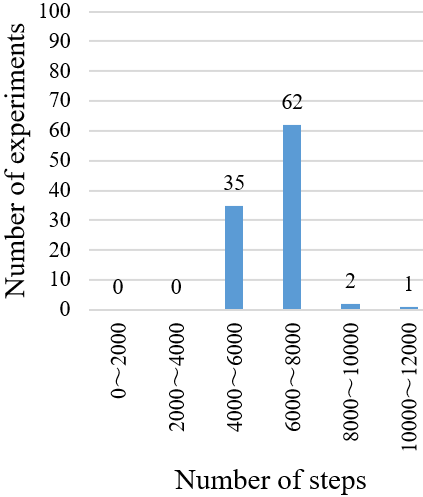
\includegraphics[keepaspectratio, scale=0.27]{./png/c.png}
    \subcaption*{\hspace*{2.5zw}(a) Conventional method}
  \end{minipage}
  \begin{minipage}[t]{0.5\linewidth}
    \centering
    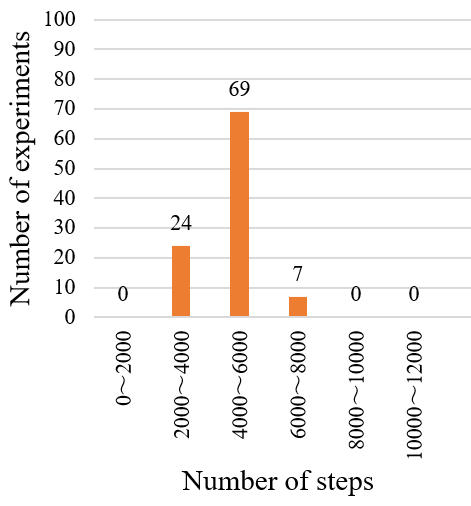
\includegraphics[keepaspectratio, scale=0.273]{./png/p.png}
    \subcaption*{\hspace*{2.5zw}(b) Proposed method}
  \end{minipage}
  \caption{Distribution of the number of steps terminated}
   \label{fig:11}
\end{figure}


\subsubsection{収集および学習したデータセットの割合}
\figref{fig:12}に収集したデータセットの割合,\figref{fig:13}に学習に用いられたデータセットの割合を示す.
これらは,従来手法と提案手法で成功した 10 回ずつの結果を平均したものである.
\figref{fig:12},\figref{fig:13}ともに,提案手法では 0 番や 1番など,直線部の割合が少なくなり,
2 番や 9 番など,曲がり角周辺の割合が多くなったことがわかる.
この結果から,収集するデータセットの偏りを改善したことで,
学習に用いられるデータセットの偏りも改善することができたといえる.
また,それにより学習を効率化できたといえる.

\begin{figure}[h!]
  \centering
   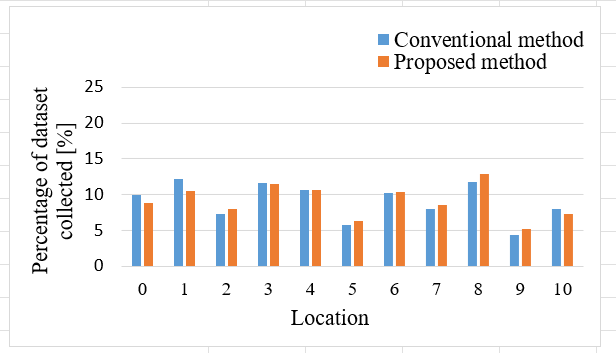
\includegraphics[height=33mm]{./png/dataset_pro2.png}
   \caption{Precentage of dataset collected}
   \label{fig:12}
\end{figure}

\begin{figure}[h!]
  \centering
   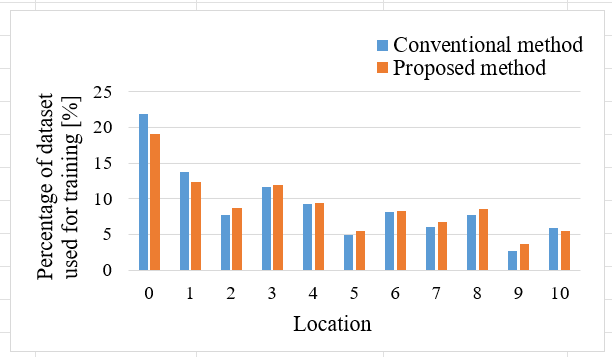
\includegraphics[height=33mm]{./png/gaku_pro2.png}
   \caption{Precentage of dataset used for training}
   \label{fig:13}
\end{figure}

\newpage

\section{結言}
本稿では,従来から提案する経路追従行動の模倣手法における経路追従失敗の一例を取り上げ,
その要因がデータセットの不均衡によるものであることを明らかにした.
そのうえで,ロボットの並進速度を教師データの値に応じて可変にすることで,データセットの収集密度を調整
し,学習を効率化する手法を提案した.その後,シミュレータでの実験により提案手法の有効性を検証した.
結果的に,提案手法は従来手法に比べて,データの不均衡を改善し,訓練打ち切りの指標を
早くに満たすことができる傾向が見られた.ただし,従来手法と提案手法で経路追従の成功率は
変わらなかったため,失敗の要因はデータセットの不均衡以外にも存在する可能性がある.もしくは,
データセットの不均衡をさらに改善する手法が必要であると考えられる.
これについては,今後の課題とする.
訓練を打ち切る指標を早く満たすことができるという点においては,提案手法は有効であることが確認された.\\

\vspace*{0.5zh}

\footnotesize
\begin{thebibliography}{99}

\bibitem{okada}
岡田眞也, 清岡優祐, 上田隆一, 林原靖男,“視覚と行動の end-
to-end 学習により経路追従行動をオンラインで模倣する手法
の提案”,計測自動制御学会 \textit{SI} 部門講演会 \textit{SICE-SI2020} 予稿
集, pp.1148-1152, 2020.

\bibitem{okada2}
岡田眞也, 清岡優祐, 春山健太, 上田隆一, 林原靖男, “視覚と
行動の end-to-end 学習により経路追従行動 をオンラインで
模倣する手法の提案 -経路追従行動の修正のためにデータセッ
トを動的に追加する手法の検討-”, 計測自動制御学会 SI 部門
講演会 SICE-SI2021 予稿集, pp.1066-1080, 2021.

\bibitem{kiyooka}
清岡優祐, 岡田眞也, 岩井一輝, 上田隆一, 林原靖男, “視覚と行動の end-
to-end 学習により経路追従行動 をオンラインで模倣する手法の提案 -データセットと
生成された経路追従行動の解析-”, 計測自動 制御学会 SI 部門講演会 SICE-SI2021 
予稿集, pp.1071-1075, 2021.

\bibitem{off_load}
U. Muller, J. Ben, E. Cosatto, B. Flepp, and Y. Cun.
“Off-Road Obstacle Avoidance through End-to-End Learning.”
Advances in neural information processing systems,
Vol. 18, 2005.

\bibitem{Moridian}
Moridian, Barzin, Anurag Kamal, and Nina Mahmoudian. 
“Learning Navigation Tasks from Demonstration for Semi-autonomous Remote
Operation of Mobile Robots.” 2018 IEEE International Symposium on
Safety, Security, and Rescue Robotics (SSRR), pp.1-8, 2018.

\bibitem{Bojarski}
Bojarski, Mariusz, \textit{et al}.,
“End to end learning for self-driving cars,” arXiv:1604.08316, 2016.

\bibitem{imai}
今井悠月 , 清岡優祐 , 春山健太 , 上田隆一 , 林原靖男 . ” 視覚と行動の end-to-end 学習によ
り経路追従行動をオンラインで模倣する手法の提案
ー経路への復帰行動の解析と復帰
行動を強化する教師データ収集法の検討ー . 日本機械学会ロボティクス・メカトロニクス
講演会 ’23 予稿集 , 2P2-G05(2023).

\bibitem{fuji}
藤原柾,春山健太,馬場琉生,上田隆一,林原靖男,"視覚と行動のend-to-end 学習により経路追従行動を
オンラインで模倣する手法の提案 実環境における経路選択機能の検証と学習時間の短縮化の検討"
,日本機械学会ロボティクス・メカトロニクス講演会'23予稿集,2P2-G06(2023)


\bibitem{takahashi}
\CID{8705}橋祐樹,白須和暉,藤原柾,上田隆一,林原靖男,"視覚と行動のend-to-end 学習による経路追従行動の模倣",
日本機械学会ロボティクス・メカトロニクス講演会'23予稿集,2P1-G07(2023)

\bibitem{imai2}
今井悠月,落合拓海,白須和暉,上田隆一,林原靖男,”視覚と行動のend-to-end 学習により経路追従行動を
オンラインで模倣する手法の提案 モデルの評価に基づく訓練ステップ数の決定”,1B1-04,SI2023,(2023)

\bibitem{navigation}
ros-planning, navigation リポジトリ\\
https://github.com/ros-planning/navigation.\\
( 最終閲覧日 : \today )

\bibitem{gazebo}
Nathan Koenig and Andrew Howard, “Design and use paradigms for gazebo, an
open-source multi-robot simulator,” \textit{2004 IEEE/RSJ International Conference
on Intelligent Robots and Systems (IROS)}, Vol.3, pp.
2149-2154, 2004.

\bibitem{TurtleBot3}
Erico Guizzo and Ackerman Evan, “The TurtleBot3 Teacher [Resources Hands On],
” \textit{IEEE Spectrum}, Vol.54, pp.19-20, August 2017.


\end{thebibliography}

\normalsize
\end{document}
